

\section{Ansaldo STS}
\subsection{System architecture}
\frame
{
  \frametitle{Ansaldo STS System architecture}
 \begin{center}
	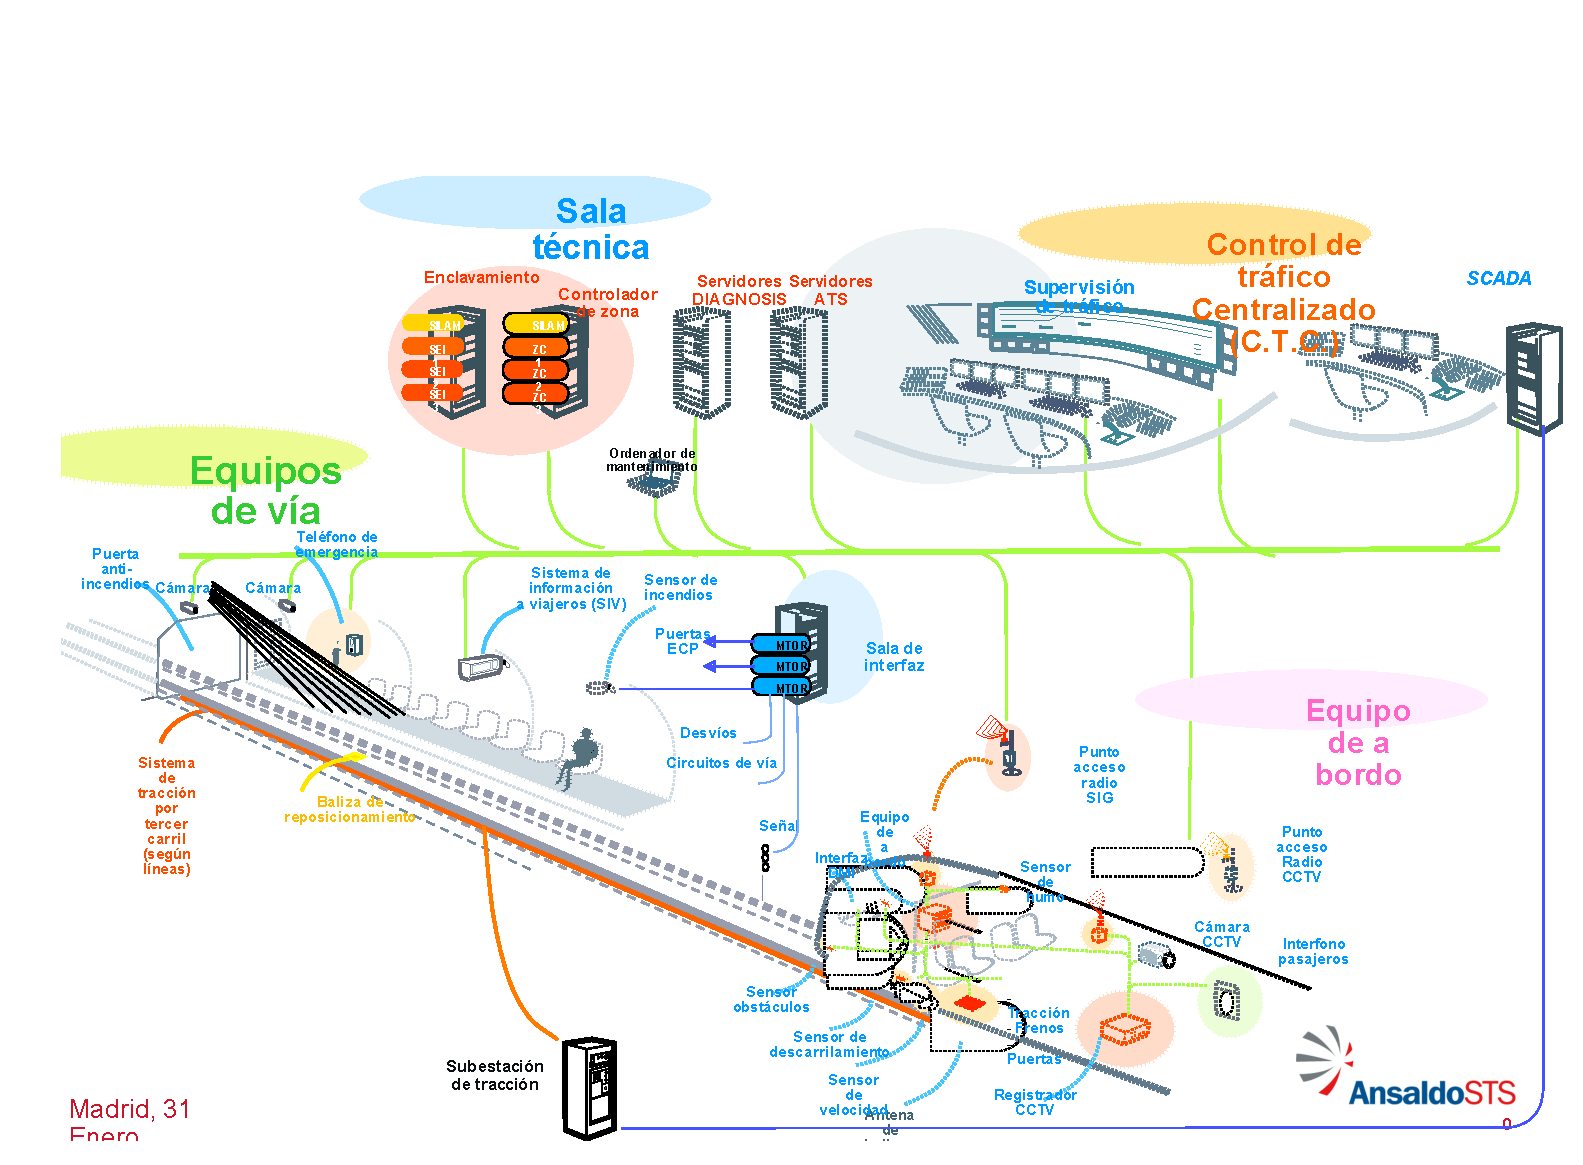
\includegraphics[scale=0.4]{./fig/AnsaldoSPsystem}
      \end{center}
   
}

\frame
{
%  \frametitle{Ansaldo STS System architecture}
 \begin{center}
	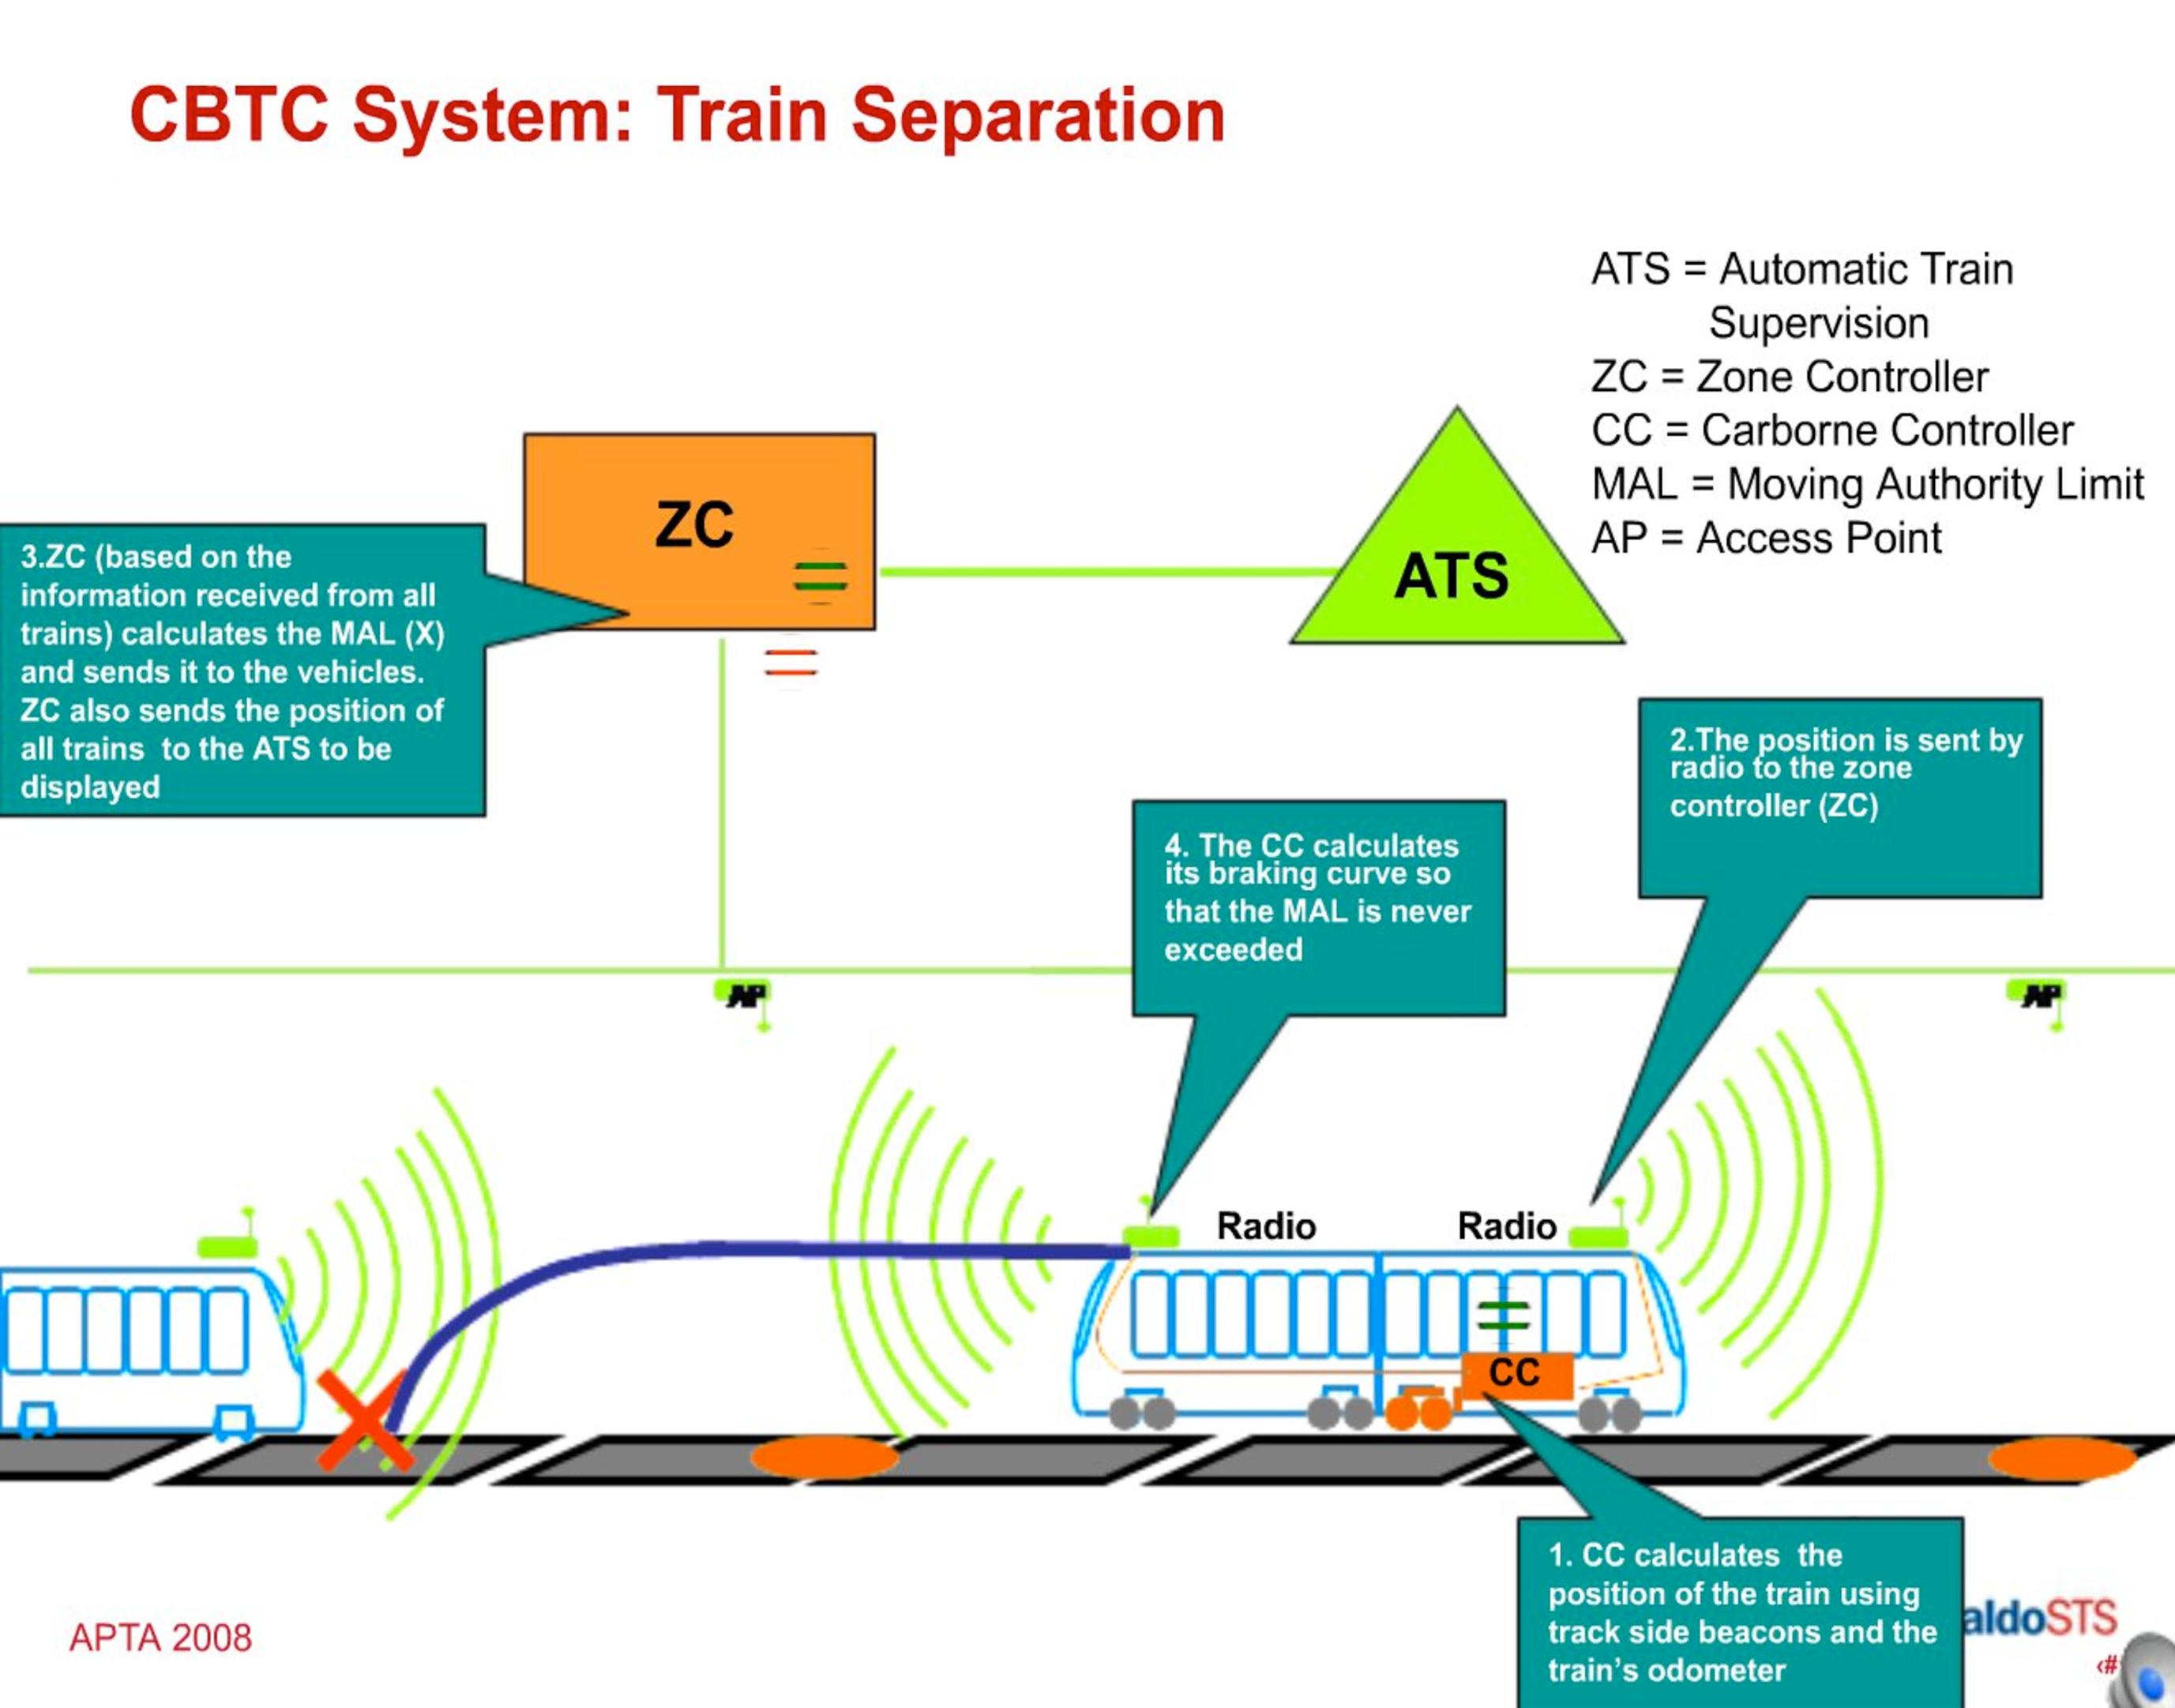
\includegraphics[scale=0.20]{./fig/AnsaldoTrainSepa}
      \end{center}
  
}


\subsection{Operating mode, Headway and Communication}
\frame
{
\begin{block}<1->{Operating mode management}
simultaneous CBTC and non-CBTC equipped vehicles to share the same tracks
\end{block}

\begin{block}<2->{Communication infrastructure and protocol}
\begin{itemize}
\item  \textbf{Train-wayside protocol} Radio Frequency: IEEE 802.11 
\item  \textbf{Fully redundant} configurations.
\end{itemize}
\end{block}
\begin{block}<3->{Headway}
\begin{itemize}
\item In brochures headway is declared down to \textbf{60s}.
\item Copenhagen Metro  \textbf{90s/100s} minimum.
\item  Taipei Circular Line \textbf{90s} minimum.
\end{itemize}

   \end{block}

}


\subsection{Safety and failure management}
\frame
{
\frametitle{Safety and failure management}
 \begin{center}
	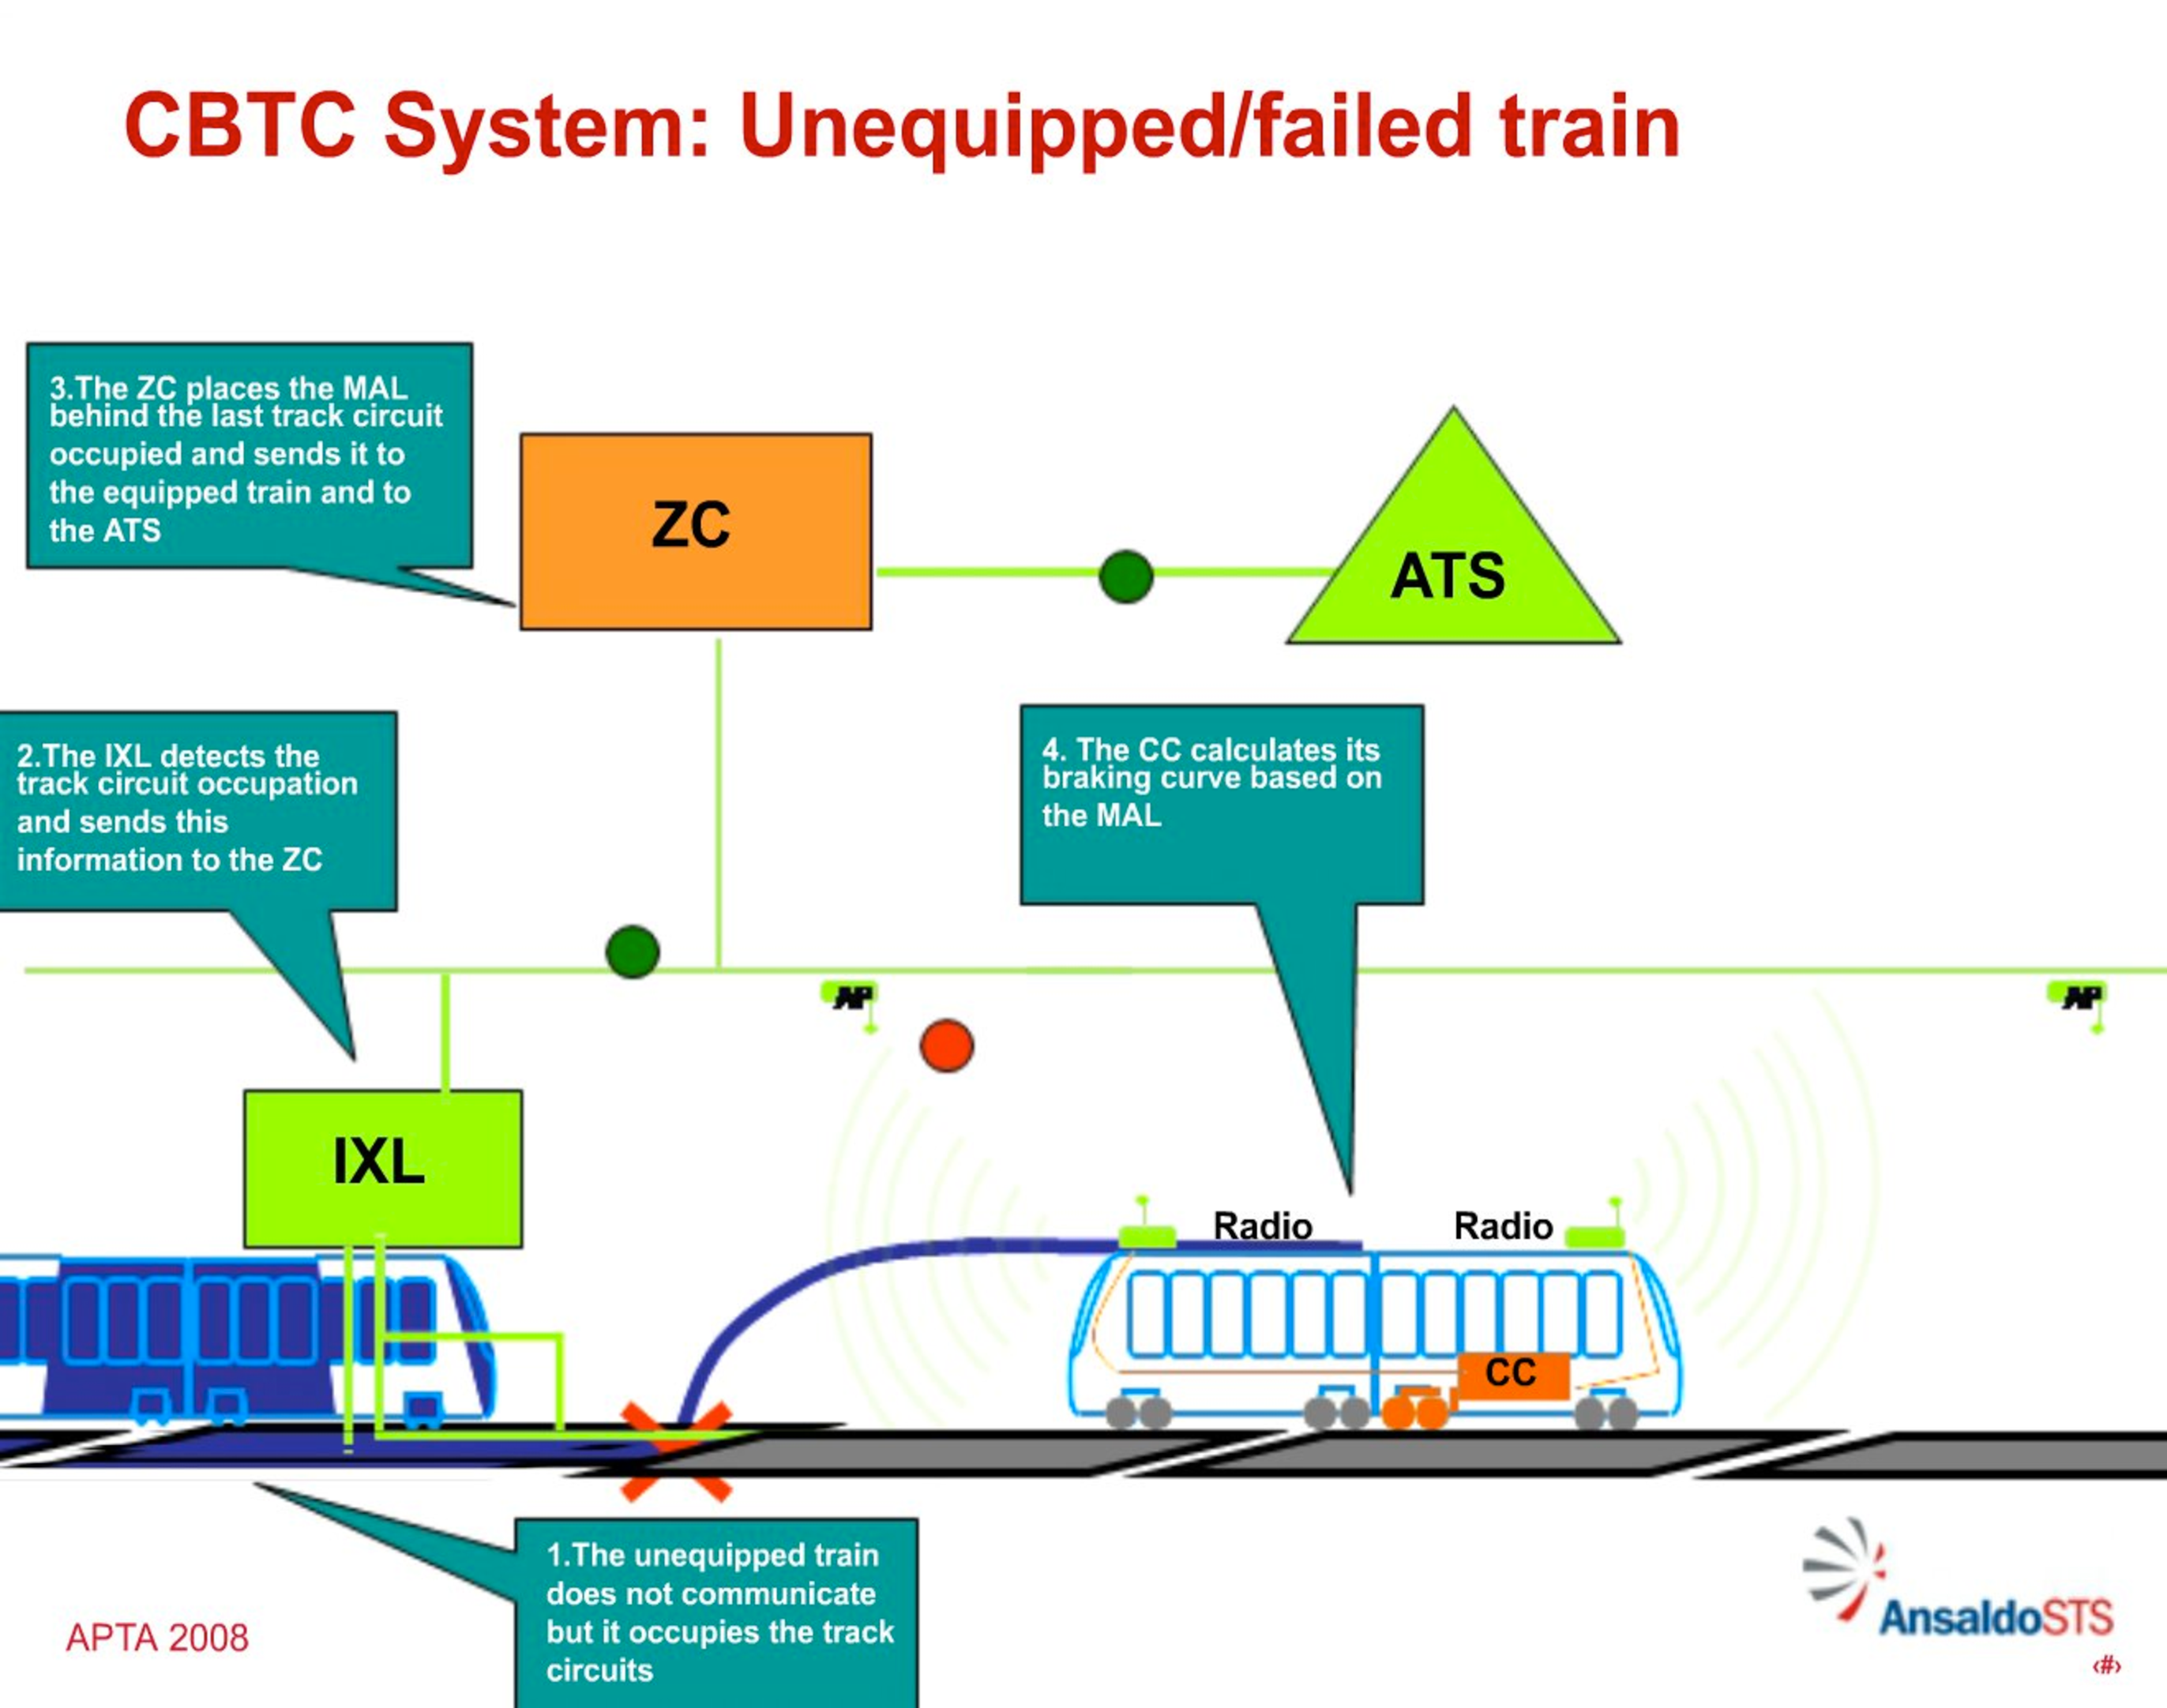
\includegraphics[scale=0.20]{./fig/AnsaldoUnequiped}
      \end{center} 


}

%System architecture
%Operating mode management
%Safety and failure management
%Communication infrastructure and protocol
\subsection{Interlocking}
\frame
{
\frametitle{Interlocking and wayside information integration}



 \begin{center}
	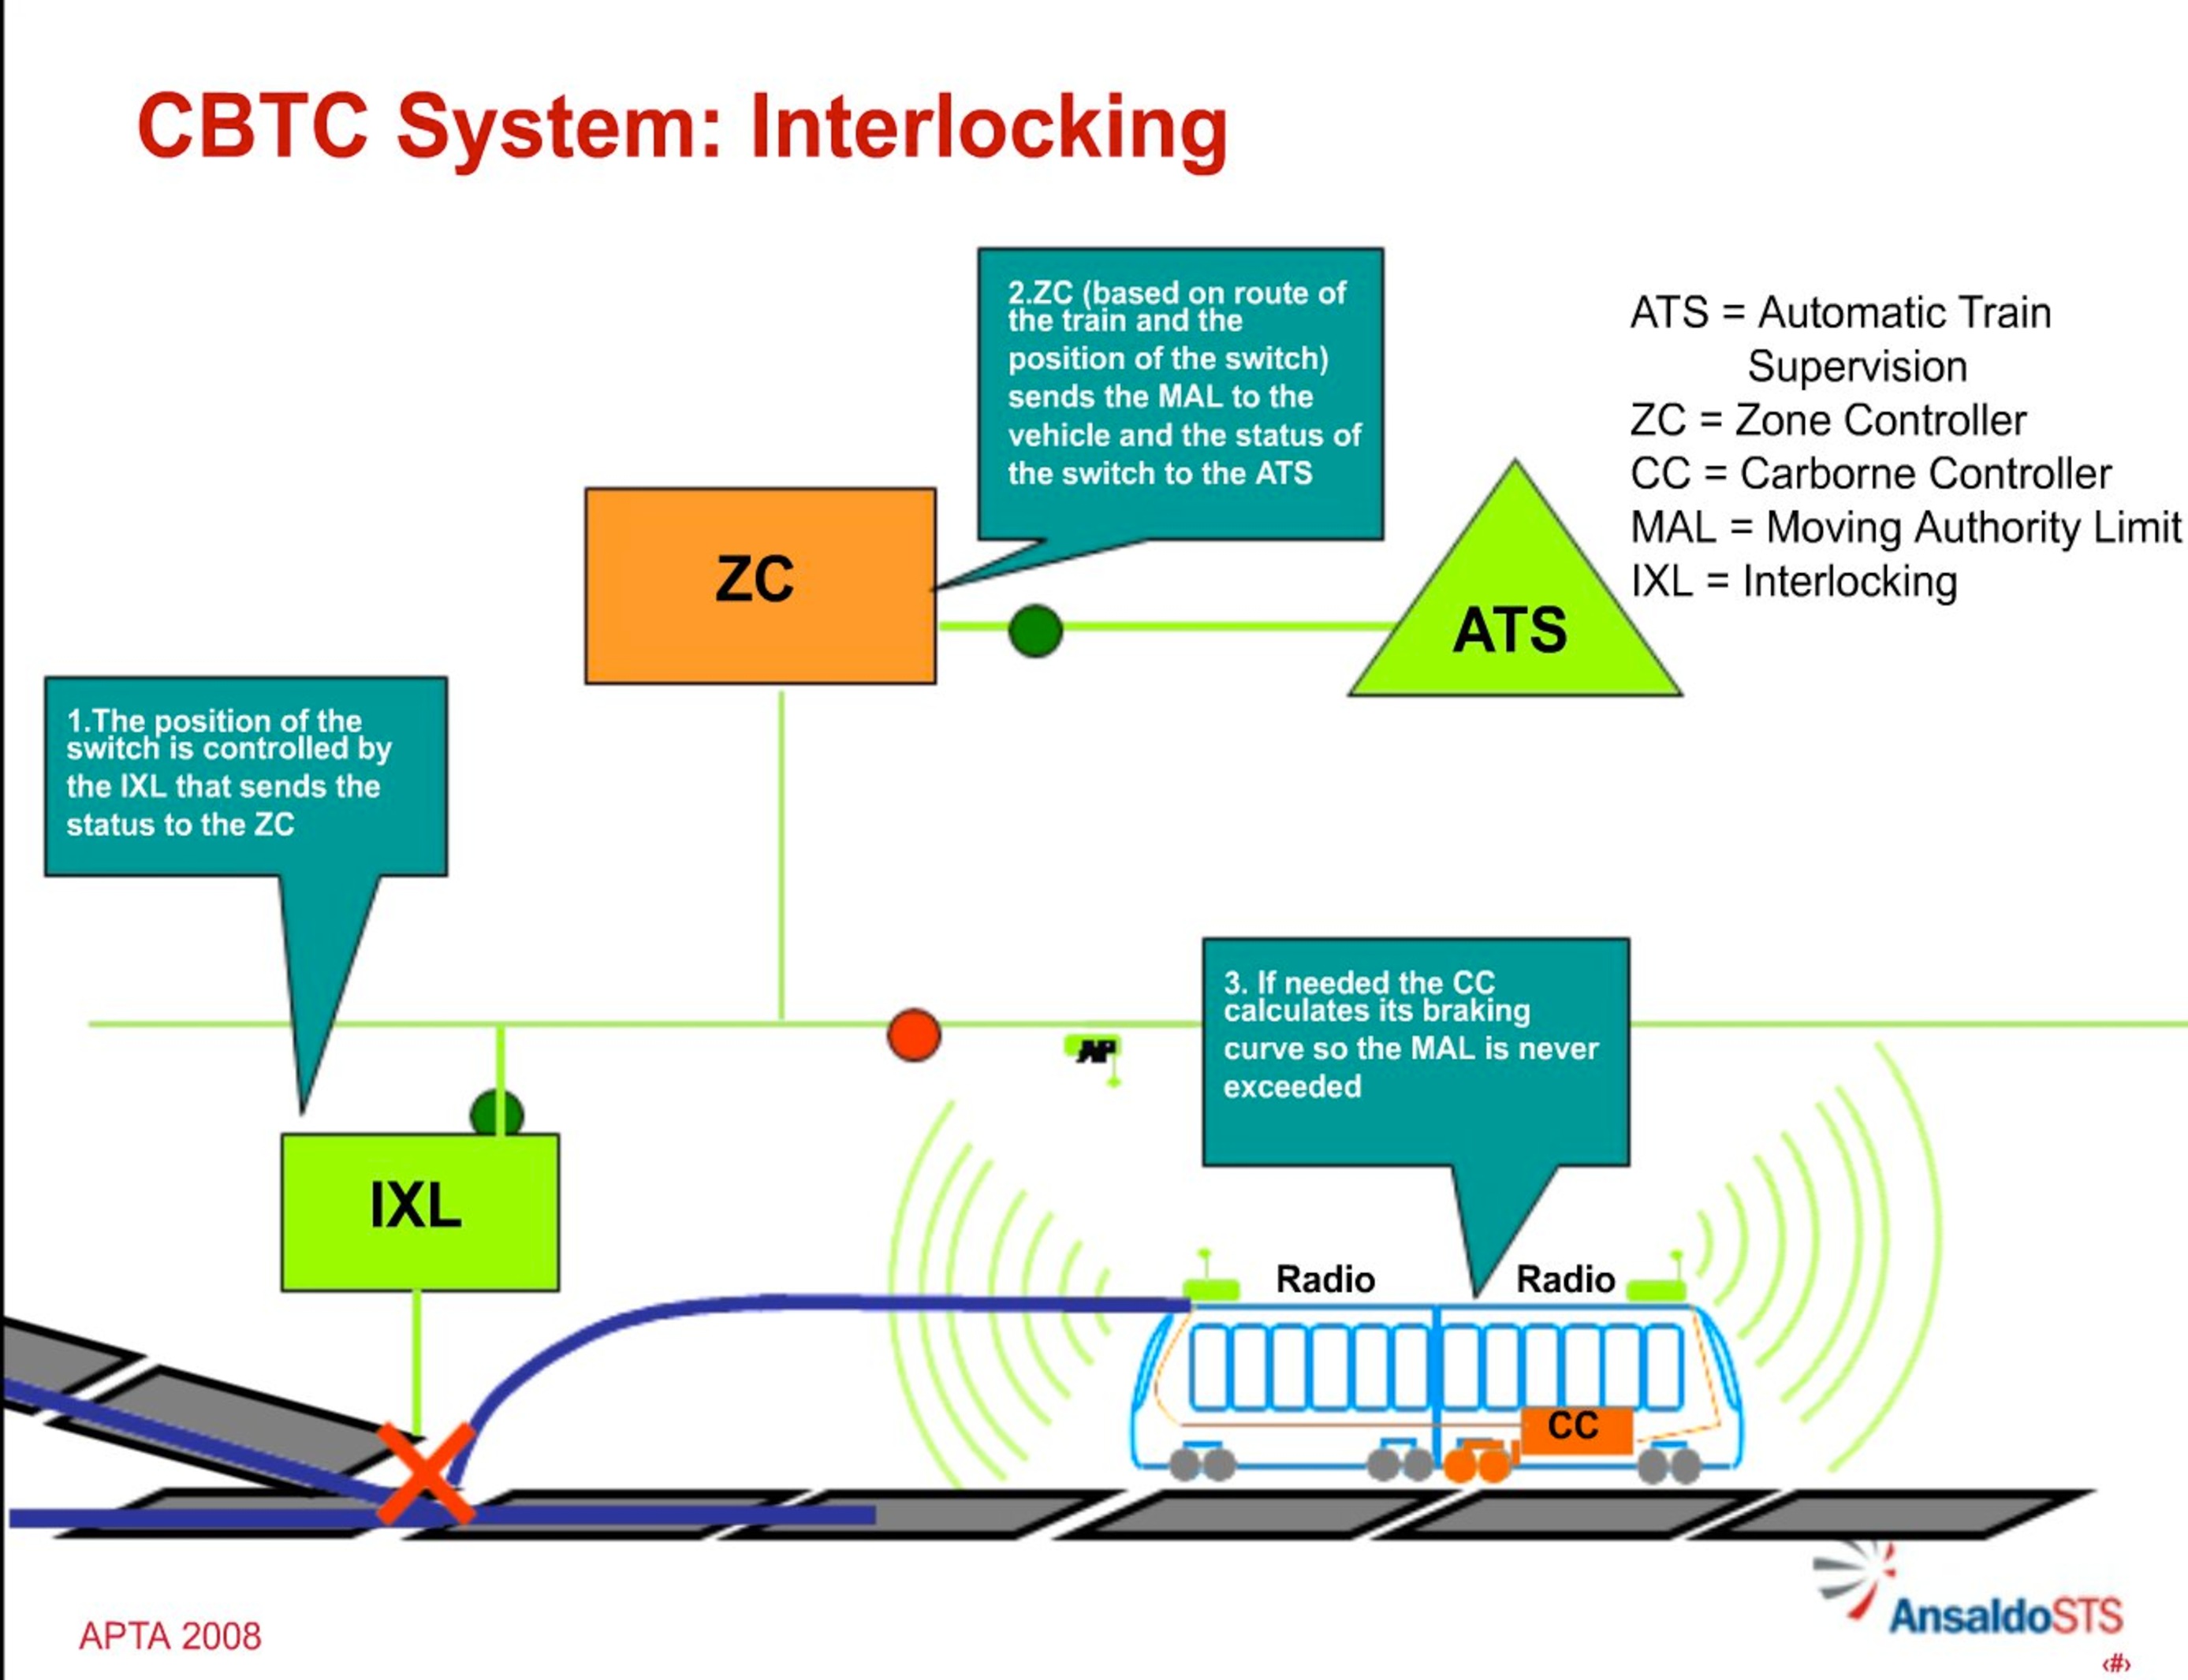
\includegraphics[scale=0.20]{./fig/AnsaldoInterloking}
      \end{center} 


  }

%Interlocking and wayside information integration

\subsection{ATS functions}
\frame
{

  
\begin{block}<1->{ATS functions}
No Information
\end{block}
   \begin{block}<1->{Braking models and speed limit protection}
No Information

   \end{block}
   
      \begin{block}<2->{Train speed and train location determination}
      \begin{itemize}
      \item The position train is determinate with use \textbf{track side beacon} to receive the absolute position and on board \textbf{odometer system} 
      \item The maximum train speed is \textbf{80km/h} into Copenhagen and Chengdu.
\end{itemize}
  \end{block}
}


%ATS functions

%\subsection{ Train speed and train location determination }
%\frame
%{
  


   




 
%}

%Headway
%Braking models and speed limit protection
%Train speed and train location determination

\subsection{Door management, ATO functions and Service-oriented facilities}
\frame
{
  

\begin{block}<1->{Door management}
\begin{itemize}
\item Door control functions is assigned at ATP, if opening authorization is true.
\item The ATO functions allows you to make small movements to center doors (\textbf{Undershoot \& Overshoot} recovery)
\end{itemize}

   \end{block}
   
   \begin{block}<2->{ATO functions}
   \begin{itemize}
\item Speed regulation
\item Management of programmed stops
\item Management of Platform Screen doors
\item Skip Stop
\item Management of overshoot ad undershoot
\item Automated coupling \& decoupling
\item Energy consumption management and optimization
%\item Routine maintenance reporting can be provided direct to the interlocking technician terminal.
\end{itemize}
   \end{block}
   
   }


%Door management
%ATO functions

\subsection{Service-oriented facilities}
\frame
{  
   
      \begin{block}<1->{Service-oriented facilities}
      \begin{itemize}
       \item Closed Circuit TV.
\item Obstacle detection system
\item Loudspeakers in stations and trains.
\item Information displays in stations and trains.
\item Emergency Call Points in stations and trains.
\end{itemize}



   \end{block}
   
    \begin{block}<2->{}
   End
   \end{block}
}

%Service-oriented facilities
%qui
  %\begin{itemize}
  %\item<1-> Normal LaTeX class.
  %\item<2-> Easy overlays.
  %\item<3-> No external programs needed.      
  %\end{itemize}

